\documentclass[11pt]{article}
\usepackage[vietnamese]{babel}
\usepackage{sectsty}
\usepackage{graphicx}
\usepackage{setspace}
\usepackage{float} 

% Margins
\topmargin=-0.45in
\evensidemargin=0in
\oddsidemargin=0in
\textwidth=6.5in
\textheight=9.0in
\headsep=0.25in

\title{STROKE PREDICTION USING MACHINE LEARNING TECHNIQUES}
\author{Khổng Đức Quang - MSSV: 20225072}
\date{\today}

\begin{document}
	\maketitle
	\textbf{TÓM TẮT}\\
	
	Con người ngày nay bị ảnh hưởng bởi nhiều loại bệnh tật do tác động của tình trạng môi trường và sự lựa chọn lối sống của con người. Việc phát hiện và lựa chọn các giải pháp phòng tránh bệnh là rất quan trọng để ngăn ngừa chúng tiến triển tới giai đoạn cuối. Đột quỵ là một trong nhwuxng nguyên nhân gây tử vong hàng đầu và là gánh nặng tài chính cho người bệnh.
	
	Chính vì lý do đó trên mà em quyết định lựa chọn chủ đề này cho học phần Project I. Để xử lý bài toán, em sử dụng bộ dữ liệu "Stroke Prediction Dataset" có sẵn trên Kaggle. Bộ dữ liệu bao gồm 5110 hàng và 12 cột thuộc tính, được xử lý trước để phù hợp với dự đoán
	
	\pagebreak
	
	\textbf{Danh sách các từ viết tắt}\\
	
	\begin{tabular}{l l}
		
		\vspace{0.25cm}
		AI  & Artificial Intelligence \\
		\vspace{0.25cm}
		DT  & Decision Tree \\
		\vspace{0.25cm}
		KNN & K-Nearest Neighbor \\
		\vspace{0.25cm}
		ML  & Machine Learning \\
		\vspace{0.25cm}
		RF  & Random Forest \\
		\vspace{0.25cm}
		SVM & Super Vector Machine \\
		\vspace{0.25cm}
	\end{tabular}
	
	% Optional TOC
	% \tableofcontents
	% \pagebreak
	
	%--Paper--
	\pagebreak
		
	
	\section{Mô tả bộ dữ liệu}
	
	
	Bộ dữ liệu được em thu thập từ trang Web Kaggle để ước tính xem bệnh nhân có khả năng đột quỵ hay không. Đâu là bộ dữ liệu về thông tin của 5110 người bao gồm 11 thuộc tính và 1 cột stroke(output) là có khả năng đột quỵ hay không. (FEDESORIANO 2021). 
	
	Dưới đây là danh sách các thuộc tính:
	\begin{enumerate}
		\item Id (Interger Feature): Đây là dữ liệu kiểu số nhằm. Tuy nhiên thuộc tính này không làm ảnh hưởng tới Output nên em sẽ không phân tích thêm.
		\item Gender (Nominal Feature): Đây là thuộc tính kiểu chữ bao gồm các giá trị: Male, Female, Orther. Thuộc tính "Gender" (giới tính) có thể ảnh hưởng tới khả năng đột quỵ do sự khác biệt sinh học, nội tiết tố, và yếu tố hành vi giữa nam và nữ.
		\item Age (Interger Feature): Dữ liệu kiểu số. Thuộc này này là một yếu tố quan trọng ảnh hưởng đến khả năng đột quỵ.
		\item Hypertension (Integer Feature): Với hai giá trị khác nhau là: 0, 1.
		Đây là yếu tố nguy cơ lớn nhất đối với đột quỵ. Nó có ảnh hưởng sâu sắc đến khả năng đột quỵ.
		\item Heart Disease (Integer Feature): Với hai giá trị khác nhau là: 0, 1. Là một yếu tố có nguy cơ đáng kể gây đột quỵ. 
		\item Ever married (Boolean Feature): Với hai giá trị khác nhau là: True, False. Có thể liên quan đến nguy cơ đột quỵ qua các yếu tố gián tiếp, chẳng hạn như lối sống, sức khỏe tâm lý, và sự hỗ trợ xã hội.
		\item Work type (Nominal Feature): Có 5 loại giá trị khác nhau: Private, Self-employed, children, Govt-job, Never-worked. Và ảnh hưởng đáng kể đến nguy cơ đột quỵ thông qua các yếu tố như mức độ căng thẳng, hoạt động thể chất, và tiếp xúc với các yếu tố nguy cơ môi trường.
		\item Residence type (Nominal Feature): Có hai giá trị khác nhau là: Urban, Rural. Ảnh hưởng đến nguy cơ đột quỵ thông qua các yếu tố môi trường, điều kiện sống, và khả năng tiếp cận dịch vụ chăm sóc sức khỏe.
		\item Avg glucose level (Float Feature): Là một yếu tố quan trọng liên quan đến nguy cơ đột quỵ, đặc biệt thông qua mối liên hệ với bệnh tiểu đường và rối loạn chuyển hóa. Mức đường huyết bất thường, cả cao lẫn thấp, đều có thể làm tăng nguy cơ đột quỵ.
		\item BMI (Float Feature): Là một chỉ số quan trọng để đánh giá mức độ béo phì hoặc thừa cân của một người, và nó có mối liên hệ mạnh mẽ với nguy cơ đột quỵ.
		\item Smoking status(Nominal Feature): Với 4 giá trị khác nhau: Never smoked, Unknown, formerly smoked, smokes. Là một yếu tố nguy cơ quan trọng đối với nhiều bệnh lý, bao gồm đột quỵ. Hút thuốc lá ảnh hưởng đến sức khỏe của tim và mạch máu, gây ra những tác động tiêu cực trực tiếp làm tăng nguy cơ đột quỵ. 
	\end{enumerate}
	
	\pagebreak
	
	\section{Xử lý dữ liệu}
	
	Trong quá trình tiền xử lý số liệu, em nhận thấy có các vấn đề sau cần xử lý:
	\begin{enumerate}
		\item Đầu tiên em \textbf{loại bỏ đi cột ID} do cột này không ảnh hưởng tới khả năng đột quỵ.
		\item
		\textbf{Xử lý các giá trị NULL}
		\begin{figure}[H]
			\centering
			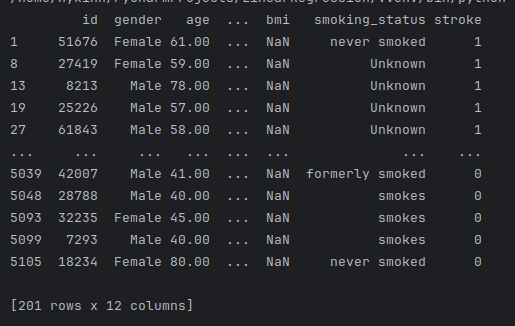
\includegraphics[width=0.7\linewidth]{nullCheck}
			\caption{Kiểm tra giá trị NULL}
			\label{fig:nullcheck}
		\end{figure}
		Sau khi kiểm tra em nhận thấy cột thuộc tính "bmi" có 201 giá trị NULL. Để xử lý vấn đề này có ba phương pháp phổ biến: Xóa các dòng chứa giá trị NULL, Điền giá trị trung bình hoặc trung vị, Điền giá trị dựa trên mô hình (Model-based Impution).
		Sau khi tìm hiểu ưu và nhược điểm của từng phương pháp em quyểt định lựa chọn cách điền giá trị trung bình là lựa chọn vừa đơn giản vừa hiệu quả, giúp giữ được lại toàn bộ dữ liệu mà không làm giảm kích thước bộ dữ liệu.
		\item Bước tiếp theo là \textbf{chuyển đổi dữ liệu kiểu Categorical thành dữ liệu kiểu Numerical}. Phương pháp Hash e Encoding và One-hot Encoding được sử dụng để thực hiện các bước chuyển đổi này.
		\item \textbf{Phân chia dữ liệu}: Em chia bộ dữ liệu thành hai tập là: tập huấn luyện(80\%), tập kiểm tra(20\%) bằng cách sử dụng hàm train\_test\_split được cung cấp trong thư viện scikit-learn
		\item \textbf{Feature scaling (chuẩn hóa đặc trưng)} là bước cuối cùng
	%--/Paper--
	\end{enumerate}
\end{document}
